% COS598 Project Paper
% Authors: Aaron Doll, Shaheed Chagan, Michael Kranch, Vaidhyanath Murti
%%%%%%%%%%%%%%%%%%%%%%%%

\documentclass[10pt, letterpaper, twocolumn, twoside]{article}
%\usepackage{epstopdf}
%\usepackage[pdftex]{graphicx}
%\usepackage[left=.8in,top=.8in,right=.8in,bottom=.8in,nohead,nofoot,columnsep=20pt]{geometry}
\usepackage[left=1in,top=1in,right=1in,bottom=1in,columnsep=20pt]{geometry}
\usepackage{setspace}
\usepackage[small,compact]{titlesec}
\usepackage{subfigure}
%\usepackage{multicol}
%\usepackage{multirow}
\usepackage{textcomp}
\usepackage{mathtools}
\usepackage{amsmath}
\usepackage[hyphens]{url}
\usepackage{float}
%\usepackage{fancyhdr}
%\setlength{\headheight}{14.5pt}
%\setlength{\footskip}{11pt}
%\pagestyle{fancy}
%\lhead{}
%\chead{}
%\rhead{}
%\rfoot{}

\newcommand{\tc}{\textcolor}

\makeatletter
\setlength{\@fptop}{0pt}
\makeatother


%make title bold and 14 pt font (Latex default is non-bold, 16 pt)
\title{\bf BTCTrackr}
\author{Aaron Doll, Shaheed Chagan, Michael Kranch, and Vaidhyanath Murti\\
\textit{\{adoll, schagani, mkranch, and vmurt\} @cs.princeton.edu}}
\date{COS 597B Privacy \\ 14 May 2014}

\begin{document}

\maketitle

% suppress page numbers
\thispagestyle{empty}

\begin{abstract}
Bitcoin is the mostly widely known and accepted of a rapid growing set of online, virtual crypto-currency. Many users are attracted to these new crypto-currencies because they are decentralized and separated from any sovereignty or authority. They are also adopting crypto-currencies because they provide pseudonymity - an individual can make online transactions with the virtual currency without any direct link to their real world identity. Because of this psuedonymity, many users believe they can use freely without risk of their expenditures being traced back to their real identity; however, several recent papers on bitcoin transactions increase demonstrate this belief is false. An individual's spending habits are actually more easily tracked by non sophisticated advisory due to the public nature of the bitcoin transaction ledge than more commonly accepted online payment methods like credit cards. Continuing on the work presented in "A Fistful of Bitcoins", this paper revisits the heuristics for identifying a individuals closure, or the subset of link Bitcoin. We then implement these heuristics in a real-time application made open to the public to allow individuals to avoid linking transactions. Finally, we discuss several other related project and future areas for improvement.

\end{abstract}

\section{Introduction}
\label{intro}
In this section, we present a brief overview of technical aspect of Bitcoin. We then several known methods of linking Bitcoin addresses presented in previous work. Finally, we discuss issue with this methods and the motivation for a real-time heuristic utility. 

\subsection{Bitcoin}
Bitcoin is an experimental, decentralized digital currency that uses peer-to-peer technology to operate with no central authority. Bitcoins are sent from one address to another with each user potentially having many, many addresses. Each payment transaction is cryptographically signed by the owner to prevent illegitiment spending and then broadcast across the peer-to-peer network to included in the list of previous transactions (more commonly known as the block chain). Miners are a special type of user that participates in the network. Miners are responsible for verifying the authenticity of an announced transaction based on the previous transactions in the block chain and including that transaction in the next block (update) to the block chain. Once a transaction is included in the block chain, that transaction can not be altered or reversed.\\

In the Bitcoin protocol, transactions are simply a list of addresses as inputs with a corresponding list of transactions as outputs. In addition, the sum of all the input address must be greater than or equal to the sum of all the output address with the difference being claimed by the miner (an optional small fee for publishing the transaction).  Figure \ref{fig:transaction} shows an example transaction where Alice pays Bob 12 BTC. Alice uses two address that are . She then pays Bob the 12 BTC and must pay herself back the additional 3 BTC to a third address (commonly called a charge address).

\begin{figure}
  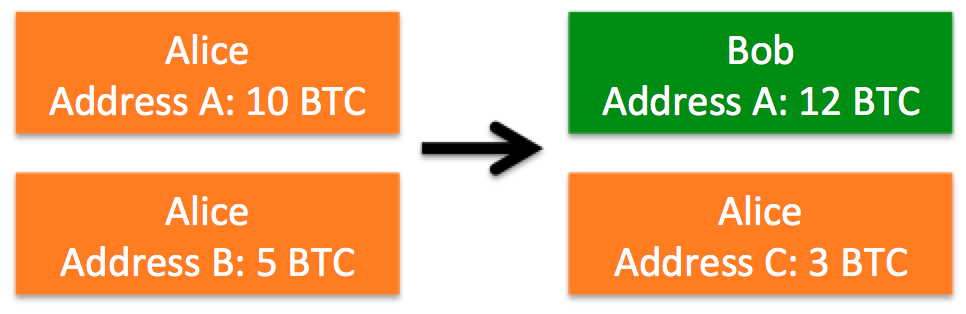
\includegraphics[width=\linewidth]{transaction.png}
  \caption{Example Transaction}
  \label{fig:transaction}
\end{figure}

\subsection{Address Clustering}

.For example, Alice might want to payindividual or entity generally controls many addresses as opposed to a traditional system where a user has a single account

Te inputs As suggested that transactions In this paper, we refer to the term clustering to mean the group (subset) of Bitcoin address that are controlled by the same individual. Furthermore, we define control as the individual in charge of spending the Bitcoins.

Heuristic one - all inputs below to same user.
Dicuss change address - 

\subsection{Motivation}
All current implementation were isolated in publicly available code but not an easy to use implementation for the everyday user. They were also not in real time and would have to be re-computed for every individual address. Finally, no one previously published or displayed a list of linked addresses. Since the closures for many large establishments are known, all


\section{BTCTrackr}

\subsection{Parser}

\subsection{Database}

\subsection{Website}

\section{Related Work}
\label{related}
The initial idea of identifying bitcoin address has been around for quite some time. This idea was first introduced in the original bitcoin paper when noted that you could assume all input addresses belonged to the same individual.

Our system was built as a real-time implementation of the Heuristics described in "A Fistful of Bitcoins" by Sarah Meiklejon etc al. 

Bit Iodine is a recently published project out of the . Spagnuolo recently published his project include a front end web service similar our deployment described in this paper.


\section{Future Work and Conclusion}



% Imports the bibliography, don't remove
\small{
\begin{thebibliography}{99}

\bibitem{libbitcoin} Maersk, N., Strateman, P., Taaki, A., and Williamson, R., ``libbitcoin - Asynchronous C++ Bitcoin library'', \emph{GitHub Repository,} 2013,
\url{http://libbitcoin.dyne.org/}.

\bibitem{fistfull} Meiklejohn, S., Pomarole, M., Jordan, G., Levchenko, K., McCoy,
D., Voelker, G. M., and Savage, S., ``A Fistful of Bitcoins: Characterizing Payments Among
Men with No Names,'' in \emph{Proceedings of the 2013 Internet Measurement Conference,} 2013, \url{http://cseweb.ucsd.edu/~smeiklejohn/files/imc13.pdf}.

\bibitem{bitcoin} Nakamoto, Satoshi, ``Bitcoin: A Peer-to-Peer Electronic Cash System,'' (2008) \url{https://bitcoin.org/bitcoin.pdf}.

\bibitem{bitiodine} Spagnuolo, Michele, ``BitIodine: Extracting Intelligence from the Bitcoin Network (Master's Thesis),' 2013, \url{https://bitiodine.net/}. 

\bibitem{znort} Znort987, ``Block Parser'', \emph{GitHub Repository,} 2012,
\url{https://github.com/znort987/blockparser}.



%P.W.D. Charles, Project Title, (2013), GitHub repository, https://github.com/charlespwd/project-title

\end{thebibliography}
}
%Bit Iodine - http://miki.it/articles/papers/#bitiodine
%Fistful of Bitcoins - cseweb.ucsd.edu/~smeiklejohn/files/imc13.pdf


\end{document}
